	\chapter{Kravspecifikation}
	
	\section{Aktør kontekst diagram}
		På figur \ref{fig:AktorKontekst} ses aktør kontekst diagrammet for Rambøll Tilsyn. Diagrammet viser, hvilke aktør der interagerer med systemet.
	\begin{figure}[H]
		\centering
		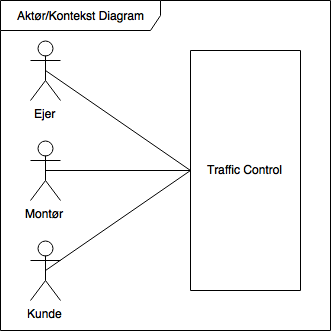
\includegraphics[width=0.6\linewidth]{Kravspecifikation/AktorDiagram}
		\caption{Aktør kontekst diagram for Rambøll Tilsyn}
		\label{fig:AktorKontekst}
	\end{figure}

		På venstre side af figur \ref{fig:AktorKontekst} ses brugeren som er den primære aktør af systemet. Brugeren benytter systemet, som på diagrammet bliver symboliseret som en blackbox. På højre side, ses de sekundære aktører. Disse aktører er dem som systemet bruger. Microsoft Office er en sekundær bruger, da systemet eksportere til Excel.
	
	\section{User stories diagram}

	\section{Funktionelle krav} 
	Følgende er en kort beskrivelse af must user stories til Rambølls Tilsyns App, som er fundet sammen med Rambøll ved hjælp af MoSCoW analyse. \cite{MoSCoW} For alle user stories fuldt beskrevet med Gherkin, se kravspecifikationen afsnit \ref{Krav-sec:UserStories}.
	Aktør kontekst diagram findes i kravspecifikationen afsnit \ref{Krav-sec:Aktor}.

	\subsection*{Log-in (CRS-1)}
	Som bruger\\
	Ønsker jeg at kunne logge ind på applikationen\\
	For at kunne benytte applikationen
	
	\subsection*{Opret bruger (CRS-2)}
	Som ejer\\
	Ønsker jeg at kunne oprette bruger på applikationen\\
	For at kunne give en ny bruger adgang til systemet
	
	\subsection*{Opret en registrering på PDF tegning (CRS-4)}
	Som bruger\\
	Ønsker jeg at kunne oprette en registrering på PDF tegning\\
	For at have kunne lave en registrering på et givet projekt 
	
	\subsection*{Opret fluebens opbjekt på PDF tegning (CRS-5)}
	Som bruger \\
	Ønsker jeg at kunne oprette et fluebens opbjekt\\
	For kunne indikere at konstruktionen er godkendt 

	\subsection*{Opret billede opbjekt på PDF tegning (CRS-6)}
	Som bruger\\
	Ønsker jeg at kunne oprette et billede objekt\\
	For at kunne tage et billede og vedlægge som dokumentation 
	
	\subsection*{Opret tekstfelt opbjekt på PDF tegning (CRS-7)}
	Som bruger\\
	Ønsker jeg at kunne oprette et tekstfelt\\
	For at kunne skrive en kommentar til en del af konstruktionen 
	
	\subsection*{Opret minus opbjekt på PDF tegning (CRS-11)}
	Som bruger\\
	Ønsker jeg at kunne oprette et minus objekt\\
	For at kunne indikere at der er en fejl konstruktionen

	\subsection*{Slet opbjekt på PDF tegning (CRS-12)}
	Som bruger\\
	Ønsker jeg at kunne slette et objekt\\
	For at kunne fjerne objekter som enten er forkerte eller en fejl 

	\subsection*{Afslut registrering på PDF tegning (CRS-13)}
	Som bruger\\
	Ønsker jeg at kunne afslutte en registrering\\
	For at kunne se en liste over tilsyns registreringerne
	
	\subsection*{Opret projekt (CRS-16)}
	Som bruger\\
	Ønsker jeg at oprette et nyt projekt\\
	For at kunne oprette nye projekter løbende
	

	\section{Ikke funktionelle krav}
	Her er nogle af systemets ikke funktionelle krav. For alle ikke funktionelle krav, se kravspecifikationen afsnit \ref{Krav-sec:Ikkefunktionelle}.
	\begin{itemize}[-]
		\itemsep 0.3em 
		\item Skal kunne tilgås gennem en Web applikation og Android applikation
		\item Der skal anvendes Microsoft teknologier og software
		\item Alle brugere skal kunne anvende systemet på samme tid. Maks antal enheder er 10 på samme tid %\\
		%\item Systemet skal have svartider under 500ms ved 99\% af requests på en dansk kablet internetforbindelse
		%\item Systemet skal have en oppetid på 99,7\%, målt over 3 måneder
		%\item Database og web-server skal være køre på hver deres server
	\end{itemize}


\section{Afgrænsning}
Projektet har en naturlig begrænsning i form af den korte tid fra idé til produkt, som er gældende for bachelorprojekter.\\
Smartphone applikationen vil blive udviklet ved anvendelse af Xamarin, det muliggør at skrive i C\# og er et cross platform SDK som gør det muligt at udvikle til både iOS og Android. \\
Applikationen som bliver udviklet til iOS i første omgang, da dette er Rambølls ønske. \\
Derudover er der til projektet lavet en Firebase database, for at mindske database problemer til udviklingen af appliaktionen og ikke påvirke Rambølls nuværende database.

\subsection{User stories, prioriteret efter MoSCoW} \label{sec:MoSCoW}
I denne sektion er der lavet en prioriteren af user stories efter MoSCoW analyse metoden.

\subsubsection{User stories}
\textbf{Must:} Log ind (CRS-1) \\
\textbf{Must:} Opret bruger (CRS-2) \\
\textbf{Must:} Opret en registrering på PDF tegning (CRS-4) \\
\textbf{Must:} Opret fluebens opbjekt på PDF tegning (CRS-5) \\
\textbf{Must:} Opret billede opbjekt på PDF tegning (CRS-6) \\
\textbf{Must:} Opret tekstfelt opbjekt på PDF tegning (CRS-7) \\
\textbf{Must:} Opret minus opbjekt på PDF tegning (CRS-11) \\
\textbf{Must:} Slet opbjekt på PDF tegning (CRS-12) \\
\textbf{Must:} Afslut registrering på PDF tegning (CRS-13) \\
\textbf{Must:} Opret projekt (CRS-16) \\

\clearpage

\textbf{Should:} Rediger af brugeroplysninger (CRS-3) \\
\textbf{Should:} Opret kommentarfelt opbjekt på PDF tegning (CRS-8) \\
\textbf{Should:} Opret pil opbjekt på PDF tegning (CRS-9) \\
\textbf{Should:} Opret cirkel opbjekt på PDF tegning (CRS-10) \\

\textbf{Could:} Opret en registrering uden PDF tegning (CRS-14) \\
\textbf{Could:} Afslut registrering uden PDF tegning (CRS-15) \\
\textbf{Could:} Rediger af projektoplysninger (CRS-17) \\
\textbf{Could:} Se tilsynsrapporter (CRS-18) \\
\textbf{Could:} Opret sub entrerpise (CRS-19)

Udfra MoSCoW analysen kan det ses hvilke user stories som der vil blive lagt fokus på først. \\
Must kategorien er den funktionalitet som skal skal implementeres under dette projekt. Should er funktionalitet som er i anden prioritet, og vil blive implementeret, hvis alle Must casene bliver færdige før afleveringsfrist. Could casene er ting som man kan arbejde videre på, hvis man ønsker at videre udvikle systemet. \\
Det forventes at alle Must casene bliver implementeret, men at Should og Could ikke bliver en del af dette projekt.
	